% fig_dt_rls_convergence.tex
% TR-43: RLS k_ibr estimation convergence
%
% X-axis: number of RLS updates (5, 10, 20, 50, 100)
% Y-axis: estimation error [%]
%
% Data from Study B:
%  updates:  5   10   20   50   100
%  error%:  6.0  2.0  3.1  1.9   0.5

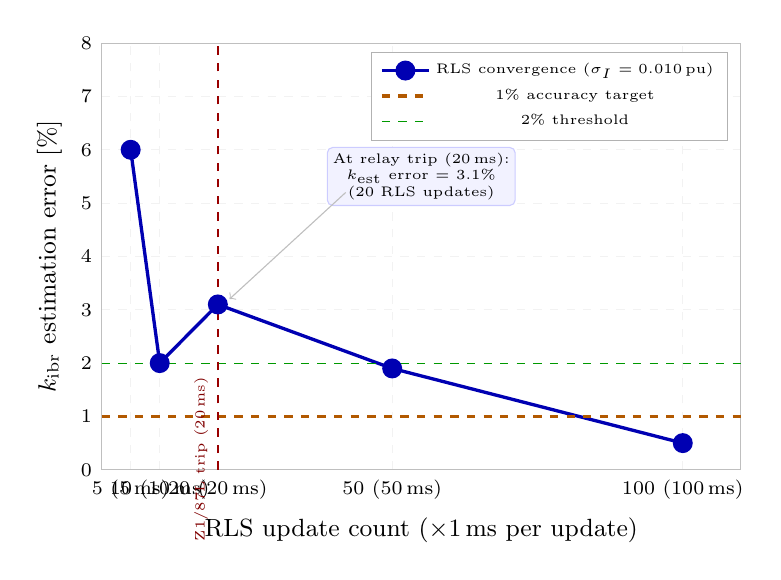
\begin{tikzpicture}
\begin{axis}[
  name         = rlsax,
  width        = 0.80\textwidth,
  height       = 7.0cm,
  xlabel       = {RLS update count ($\times 1$\,ms per update)},
  ylabel       = {$k_\mathrm{ibr}$ estimation error [\%]},
  xlabel style = {font=\small},
  ylabel style = {font=\small},
  xmin=0, xmax=110,
  ymin=0, ymax=8,
  xtick        = {5,10,20,50,100},
  xticklabels  = {5 (5\,ms), 10 (10\,ms), 20 (20\,ms), 50 (50\,ms), 100 (100\,ms)},
  xticklabel style={font=\scriptsize},
  ytick        = {0,1,2,3,4,5,6,7,8},
  yticklabel style={font=\scriptsize},
  tick style   = {draw=none},
  axis line style={gray!50},
  grid         = major,
  grid style   = {gray!10, dashed},
  legend style = {at={(0.98,0.98)}, anchor=north east, font=\tiny,
                  draw=gray!60, fill=white},
  clip=false,
]

%% RLS convergence curve
\addplot[blue!70!black, very thick, mark=*, mark size=3pt]
  coordinates {(5,6.0) (10,2.0) (20,3.1) (50,1.9) (100,0.5)};
\addlegendentry{RLS convergence ($\sigma_I=0.010$\,pu)}

%% 1% accuracy threshold
\addplot[orange!70!black, very thick, dashed]
  coordinates {(0,1.0) (110,1.0)};
\addlegendentry{1\% accuracy target}

%% 2% threshold
\addplot[green!60!black, dashed, thin]
  coordinates {(0,2.0) (110,2.0)};
\addlegendentry{2\% threshold}

%% Z1/87L trip time marker (20ms = 20 updates)
\draw[red!60!black, thick, dashed]
  (axis cs:20, 0) -- (axis cs:20, 8);
\node[red!50!black, font=\tiny, rotate=90, anchor=south]
  at (axis cs:20, 0.2) {Z1/87L trip (20\,ms)};

%% Annotation: error at trip time
\node[draw=blue!20, fill=blue!5, rounded corners=2pt,
      font=\tiny, inner sep=2pt, align=center]
  at (axis cs:55, 5.5)
  {At relay trip (20\,ms):\\
   $k_\mathrm{est}$ error = 3.1\%\\
   (20 RLS updates)};
\draw[->, gray!50, thin] (axis cs:42, 5.2) -- (axis cs:22, 3.2);

\end{axis}
\end{tikzpicture}
